\pagestyle{plain}  % kvuli cislovani

\chapter{Sada nástrojů}

\todo[inline, color=blue!30]{TODO: Rychlý úvod do všech nástrojů. Rozebrat hlavně mm-evocat, protože ten je základem návrhu. Názvy článků přidat do literatury na konci.}

\section{MM-cat}

MM-cat framework je navržený tak, aby řešil složitosti spojené s návrhem a správou multi-modelových databází. Jeho hlavním úkolem je modelování multi-modelových schémat a jejich mapování na příšlušné SŘBD (Systémy řízení bází dat). Slouží i jako základ pro rozšíření o složitější úkoly.

Typickým scénářem použití je vytvoření ER (entity-relationship) schématu uživatelem. Takové schéma je pak automaticky převedeno do jednotné kategorické reprezentace, která umožňuje namapování na kombinaci SŘBD. Díky specifikaci schématu je vytvořen skript s příkazy CREATE, které se aplikují na přiřazené SŘBD. Uživatel může následně dál upravovat ER diagram, nebo provádět SELECT dotazy.

Na ukázce uživatelského rozhraní (Obrázek \ref{obr01:mm-cat}) je výsledek typického scénáře rozebraného v předchozím odstavci. Na levé straně je uživatelem vytvořený ER diagram, na straně pravé pak jeho kategorická reprezentace. Na pravé straně ještě stojí za povšimnutí panel s přístupovými cestami (značené oranžově) a CREATE příkaz.

\begin{figure}[htb]
  \centering
  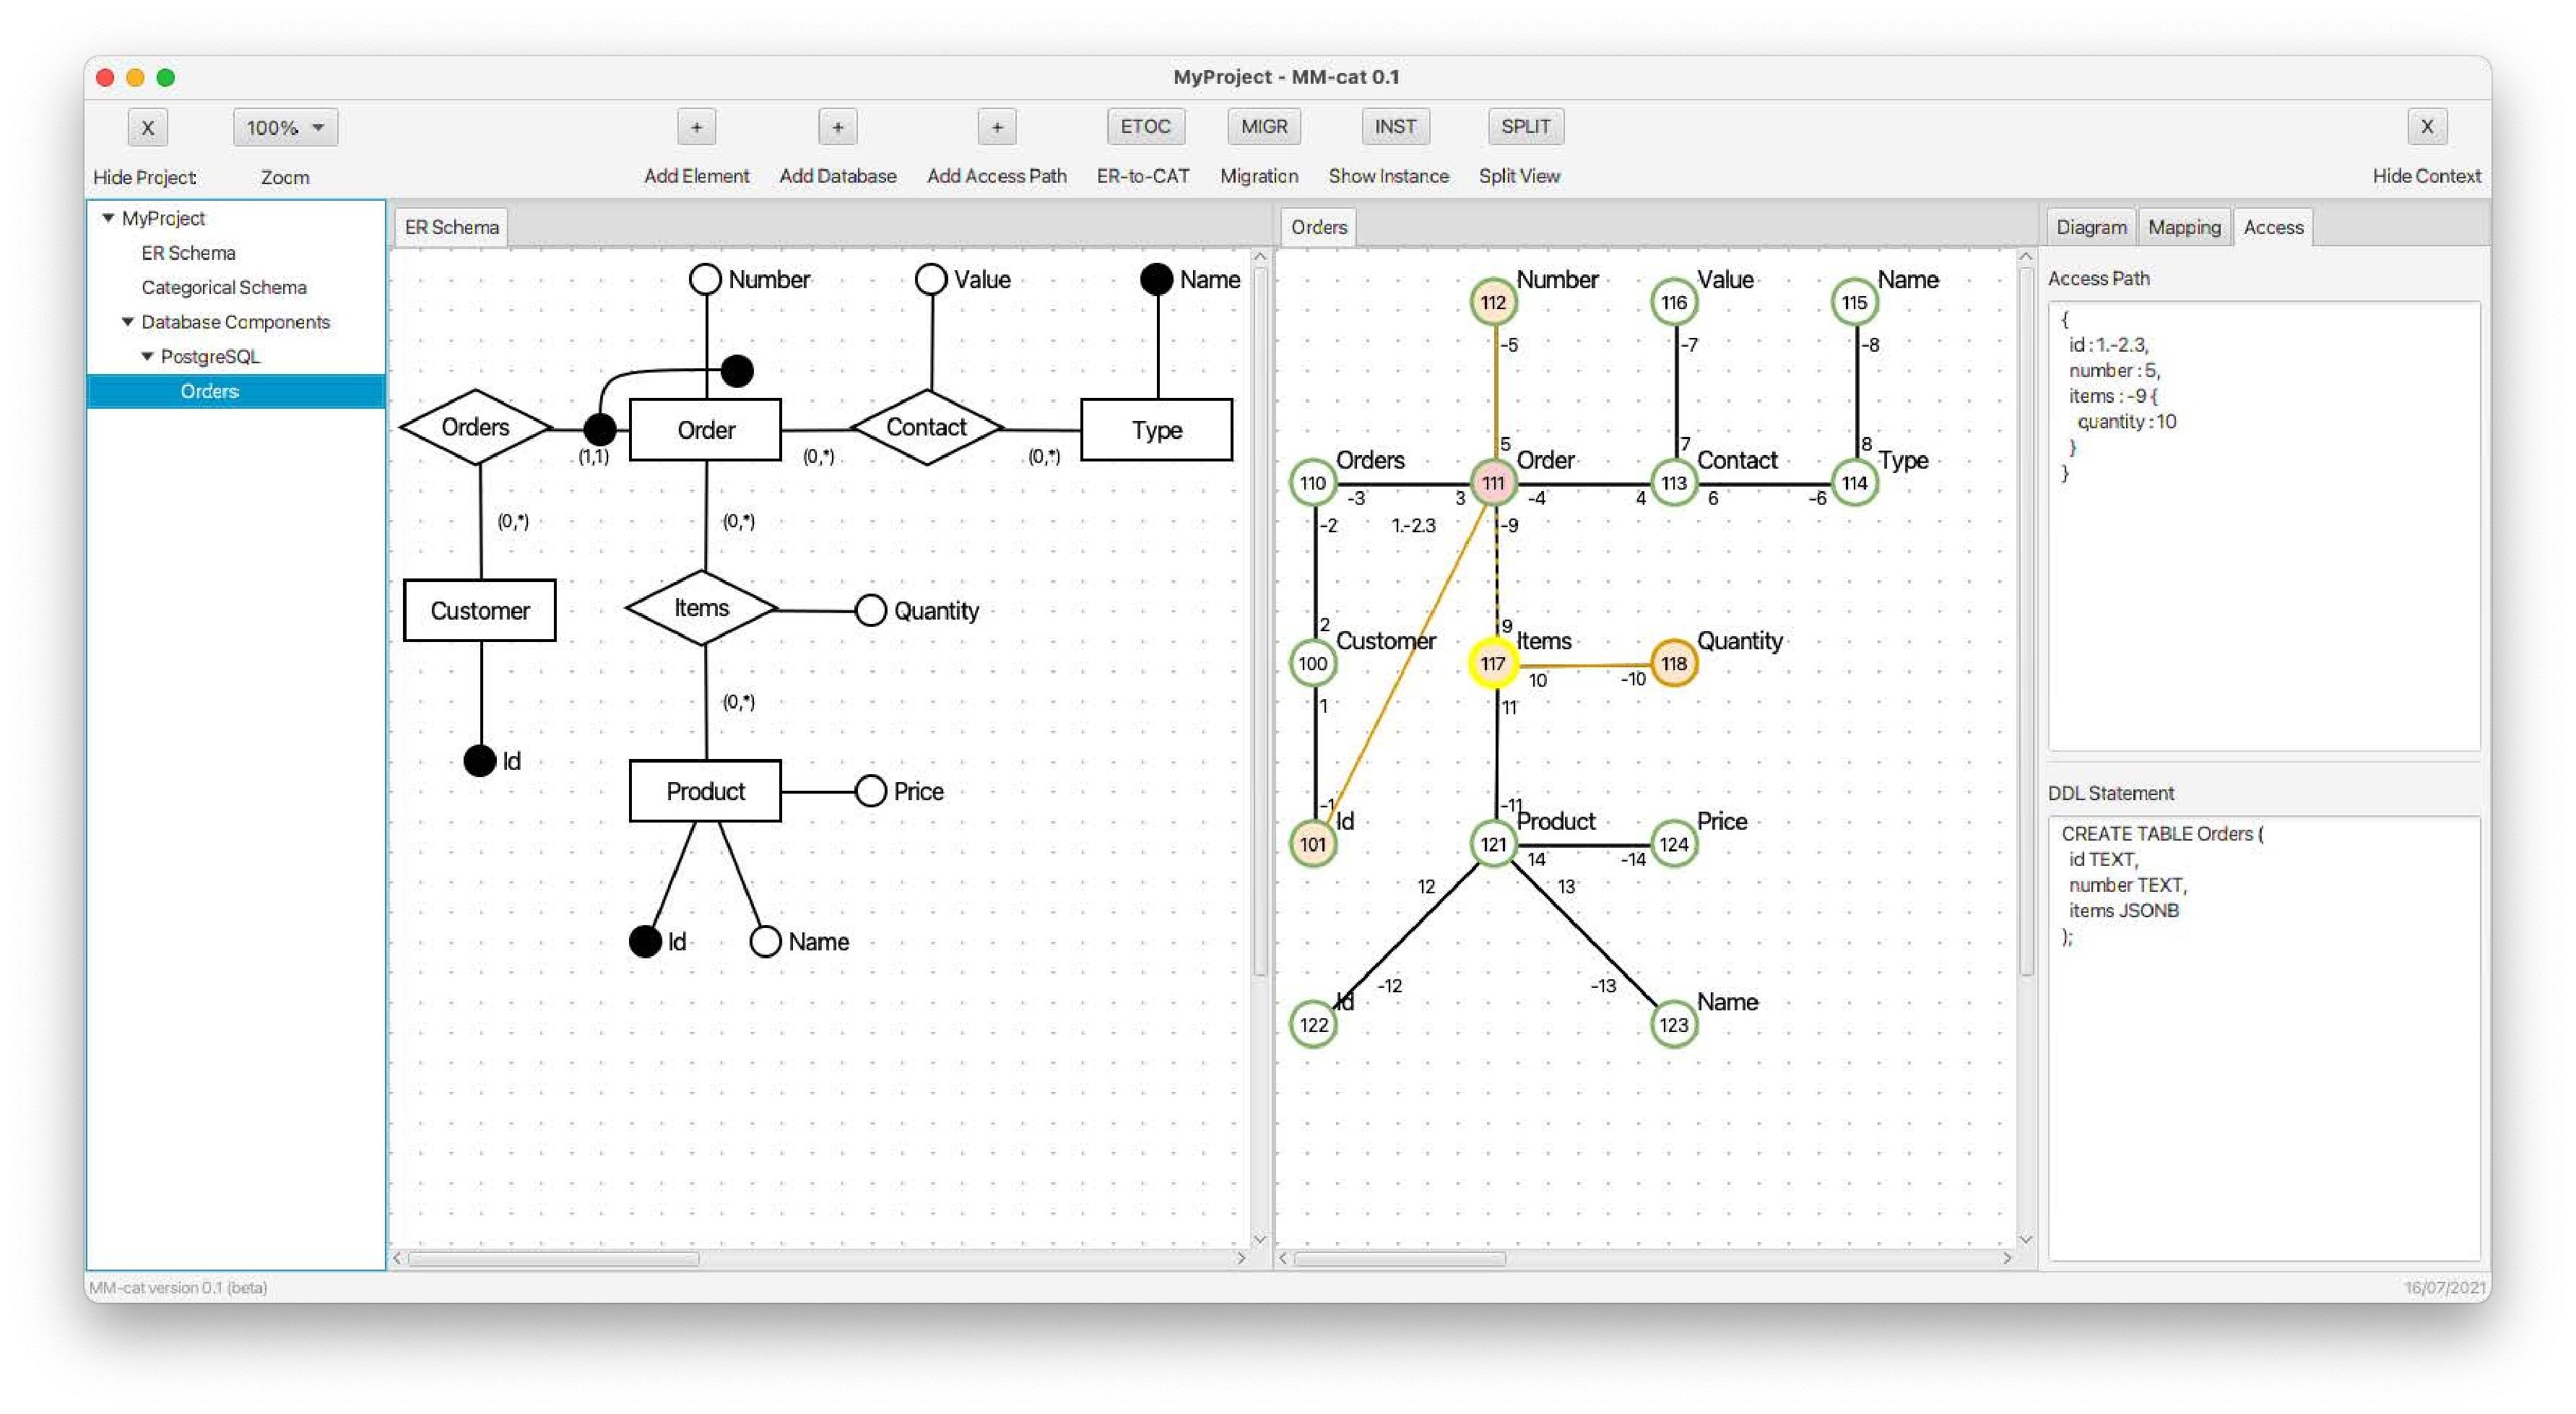
\includegraphics[height=75mm]{../img/mm-cat}
  \caption{Ukázka uživatelského rozhraní nástroje MM-cat.}
  \label{obr01:mm-cat}
\end{figure}

Další možnosti použití, i podrobnější popis nástroje, lze nalézt v článku [odkaz ->].

KOUPIL, Pavel; SVOBODA, Martin; HOLUBOVÁ, Irena. MM-cat: A tool for modeling and transformation of multi-model data using category theory. In: 2021 ACM/IEEE International Conference on Model Driven Engineering Languages and Systems Companion (MODELS-C). IEEE, 2021. p. 635-639.



\section{MM-infer}

KOUPIL, Pavel; HRICKO, Sebastián; HOLUBOVÁ, Irena. MM-infer: A Tool for Inference of Multi-Model Schemas. In: EDBT. 2022. p. 566-2.




\section{MM-evocat}

KOUPIL, Pavel; BÁRTÍK, Jáchym; HOLUBOVÁ, Irena. MM-evocat: A tool for modelling and evolution management of multi-model data. In: Proceedings of the 31st ACM International Conference on Information \& Knowledge Management. 2022. p. 4892-4896.


\section{MM-quecat}

KOUPIL, Pavel; CRHA, Daniel; HOLUBOVÁ, Irena. MM-quecat: A Tool for Unified Querying of Multi-Model Data. 2023.
